\documentclass[a4paper,justified,final,twoside,nobib]{tufte-book}

\hypersetup{colorlinks}% uncomment this line if you prefer colored hyperlinks (e.g., for onscreen viewing)

\usepackage{mathtools} %added mathtools for piecewise functions

%%
% Book metadata
\title{A\\Machine Learning\\Handbook\thanks{Thanks to Edward R.~Tufte for his inspiration.}}
\author[]{}
\publisher{Publisher of This Book}

%%
% Automated bibliography management
\usepackage{natbib}
\setcitestyle{authoryear}

%%
% If they're installed, use Bergamo and Chantilly from www.fontsite.com.
% They're clones of Bembo and Gill Sans, respectively.
%\IfFileExists{bergamo.sty}{\usepackage[osf]{bergamo}}{}% Bembo
%\IfFileExists{chantill.sty}{\usepackage{chantill}}{}% Gill Sans

\usepackage{microtype}

%%
% Describe algorithms using fancy pseudo code
\usepackage{algorithm}
\usepackage[noend]{algpseudocode}

%%
% Just some sample text
\usepackage{lipsum}
\usepackage{soul}
%%
% For nicely typeset tabular material
\usepackage{booktabs}
\usepackage{pdfpages}

%%
% For graphics / images
\usepackage{graphicx}
\setkeys{Gin}{width=\linewidth,totalheight=\textheight,keepaspectratio}
\graphicspath{{graphics/}}

% The fancyvrb package lets us customize the formatting of verbatim
% environments.  We use a slightly smaller font.
\usepackage{fancyvrb}
\fvset{fontsize=\normalsize}

%%
% Prints argument within hanging parentheses (i.e., parentheses that take
% up no horizontal space).  Useful in tabular environments.
\newcommand{\hangp}[1]{\makebox[0pt][r]{(}#1\makebox[0pt][l]{)}}

%%
% Prints an asterisk that takes up no horizontal space.
% Useful in tabular environments.
\newcommand{\hangstar}{\makebox[0pt][l]{*}}

%%
% Prints a trailing space in a smart way.
\usepackage{xspace}
% bold in maths equations
\usepackage{bm}

%%
% Some shortcuts for Tufte's book titles.  The lowercase commands will
% produce the initials of the book title in italics.  The all-caps commands
% will print out the full title of the book in italics.
\newcommand{\vdqi}{\textit{VDQI}\xspace}
\newcommand{\ei}{\textit{EI}\xspace}
\newcommand{\ve}{\textit{VE}\xspace}
\newcommand{\be}{\textit{BE}\xspace}
\newcommand{\VDQI}{\textit{The Visual Display of Quantitative Information}\xspace}
\newcommand{\EI}{\textit{Envisioning Information}\xspace}
\newcommand{\VE}{\textit{Visual Explanations}\xspace}
\newcommand{\BE}{\textit{Beautiful Evidence}\xspace}
\newcommand{\ics}{\smallcaps{ICS5110 Applied Machine Learning\xspace}}

\newcommand{\TL}{Tufte-\LaTeX\xspace}

% Prints the month name (e.g., January) and the year (e.g., 2008)
\newcommand{\monthyear}{%
  \ifcase\month\or January\or February\or March\or April\or May\or June\or
  July\or August\or September\or October\or November\or
  December\fi\space\number\year
}

% Prints an epigraph and speaker in sans serif, all-caps type.
\newcommand{\openepigraph}[2]{%
  %\sffamily\fontsize{14}{16}\selectfont
  \begin{fullwidth}
  \sffamily\large
  \begin{doublespace}
  \noindent\allcaps{#1}\\% epigraph
  \noindent\allcaps{#2}% author
  \end{doublespace}
  \end{fullwidth}
}

% Inserts a blank page
\newcommand{\blankpage}{\newpage\hbox{}\thispagestyle{empty}\newpage}

\usepackage{units}

% Typesets the font size, leading, and measure in the form of 10/12x26 pc.
\newcommand{\measure}[3]{#1/#2$\times$\unit[#3]{pc}}

% Macros for typesetting the documentation
\newcommand{\hlred}[1]{\textcolor{Maroon}{#1}}% prints in red
\newcommand{\hangleft}[1]{\makebox[0pt][r]{#1}}
\newcommand{\hairsp}{\hspace{1pt}}% hair space
\newcommand{\hquad}{\hskip0.5em\relax}% half quad space
\newcommand{\TODO}{\textcolor{red}{\bf TODO!}\xspace}
\newcommand{\ie}{\textit{i.\hairsp{}e.}\xspace}
\newcommand{\eg}{\textit{e.\hairsp{}g.}\xspace}
\newcommand{\na}{\quad--}% used in tables for N/A cells
\providecommand{\XeLaTeX}{X\lower.5ex\hbox{\kern-0.15em\reflectbox{E}}\kern-0.1em\LaTeX}
\newcommand{\tXeLaTeX}{\XeLaTeX\index{XeLaTeX@\protect\XeLaTeX}}
% \index{\texttt{\textbackslash xyz}@\hangleft{\texttt{\textbackslash}}\texttt{xyz}}
\newcommand{\tuftebs}{\symbol{'134}}% a backslash in tt type in OT1/T1
\newcommand{\doccmdnoindex}[2][]{\texttt{\tuftebs#2}}% command name -- adds backslash automatically (and doesn't add cmd to the index)
\newcommand{\doccmddef}[2][]{%
  \hlred{\texttt{\tuftebs#2}}\label{cmd:#2}%
  \ifthenelse{\isempty{#1}}%
    {% add the command to the index
      \index{#2 command@\protect\hangleft{\texttt{\tuftebs}}\texttt{#2}}% command name
    }%
    {% add the command and package to the index
      \index{#2 command@\protect\hangleft{\texttt{\tuftebs}}\texttt{#2} (\texttt{#1} package)}% command name
      \index{#1 package@\texttt{#1} package}\index{packages!#1@\texttt{#1}}% package name
    }%
}% command name -- adds backslash automatically
\newcommand{\doccmd}[2][]{%
  \texttt{\tuftebs#2}%
  \ifthenelse{\isempty{#1}}%
    {% add the command to the index
      \index{#2 command@\protect\hangleft{\texttt{\tuftebs}}\texttt{#2}}% command name
    }%
    {% add the command and package to the index
      \index{#2 command@\protect\hangleft{\texttt{\tuftebs}}\texttt{#2} (\texttt{#1} package)}% command name
      \index{#1 package@\texttt{#1} package}\index{packages!#1@\texttt{#1}}% package name
    }%
}% command name -- adds backslash automatically
\newcommand{\docopt}[1]{\ensuremath{\langle}\textrm{\textit{#1}}\ensuremath{\rangle}}% optional command argument
\newcommand{\docarg}[1]{\textrm{\textit{#1}}}% (required) command argument
\newenvironment{docspec}{\begin{quotation}\ttfamily\parskip0pt\parindent0pt\ignorespaces}{\end{quotation}}% command specification environment
\newcommand{\docenv}[1]{\texttt{#1}\index{#1 environment@\texttt{#1} environment}\index{environments!#1@\texttt{#1}}}% environment name
\newcommand{\docenvdef}[1]{\hlred{\texttt{#1}}\label{env:#1}\index{#1 environment@\texttt{#1} environment}\index{environments!#1@\texttt{#1}}}% environment name
\newcommand{\docpkg}[1]{\texttt{#1}\index{#1 package@\texttt{#1} package}\index{packages!#1@\texttt{#1}}}% package name
\newcommand{\doccls}[1]{\texttt{#1}}% document class name
\newcommand{\docclsopt}[1]{\texttt{#1}\index{#1 class option@\texttt{#1} class option}\index{class options!#1@\texttt{#1}}}% document class option name
\newcommand{\docclsoptdef}[1]{\hlred{\texttt{#1}}\label{clsopt:#1}\index{#1 class option@\texttt{#1} class option}\index{class options!#1@\texttt{#1}}}% document class option name defined
\newcommand{\docmsg}[2]{\bigskip\begin{fullwidth}\noindent\ttfamily#1\end{fullwidth}\medskip\par\noindent#2}
\newcommand{\docfilehook}[2]{\texttt{#1}\index{file hooks!#2}\index{#1@\texttt{#1}}}
\newcommand{\doccounter}[1]{\texttt{#1}\index{#1 counter@\texttt{#1} counter}}

% Generates the index
\usepackage{makeidx}
\makeindex

\usepackage{tikz}
\usepackage{makecell}

\begin{document}
%% Cover Page
\begingroup
\thispagestyle{empty}
\begin{tikzpicture}[remember picture,overlay]
\node[inner sep=0pt, outer sep=0pt] (background) at (current page.center) {\includegraphics[width=\paperwidth]{cover/cover_oreilly_style.pdf}};
\end{tikzpicture}
\vfill
\endgroup

% Front matter
\frontmatter

% r.3 full title page
%% \maketitle


% v.4 copyright page
\newpage
\begin{fullwidth}
~\vfill
\thispagestyle{empty}
\setlength{\parindent}{0pt}
\setlength{\parskip}{\baselineskip}
\begin{figure*}[h]
	\includegraphics[width=2.5in]{UMLOGO_redRGB.png}%
\end{figure*}

\par Copyright \copyright\ \the\year\ \ics\ class of 2018/9, University of Malta.

\par\smallcaps{Jean-Paul Ebejer, Dylan Seychell, Lara Marie Demajo, Daniel Farrugia, Keith Mintoff, Franco Cassar Manghi, David Farrugia, Ivan Salomone, Andrew Cachia, Jake J.\ Dalli, Joseph Azzopardi, Natalia Mallia, Mark Muscat, Stefan Cassar, Patrick Bezzina, Dylan Vassallo, Brian Pace, George Eduardo Buckup Sulzbeck, Katrin Jansen \hl{ADD YOUR NAME TO THIS LIST}} %TODO

\par Licensed under the Apache License, Version 2.0 (the ``License''); you may not
use this file except in compliance with the License. You may obtain a copy
of the License at \url{http://www.apache.org/licenses/LICENSE-2.0}. Unless
required by applicable law or agreed to in writing, software distributed
under the License is distributed on an \smallcaps{``AS IS'' BASIS, WITHOUT
WARRANTIES OR CONDITIONS OF ANY KIND}, either express or implied. See the
License for the specific language governing permissions and limitations
under the License.\index{license}

\par\textit{First printing, \monthyear}
\end{fullwidth}

% r.5 contents
\tableofcontents

%%\listoffigures

%%\listoftables

% r.9 introduction
\cleardoublepage
\chapter{Introduction}

This book explains popular Machine Learning terms.  We focus to explain each term comprehensively, through the use of examples and diagrams.  The description of each term is written by a student sitting in for \ics\footnote{\url{https://www.um.edu.mt/courses/studyunit/ICS5110}} at the University of Malta (class 2018/2019).  This study-unit is part of the MSc.\ in AI offered by the Department of Artificial Intelligence, Faculty of ICT.

%%
% Start the main matter (normal chapters)
\mainmatter

%% JP's example file -- file must be stored in directory "terms" and have
%% the term and initials of the student in the filename.
\input{terms/activationfunctions_km.tex}
\chapter{Bayesian Models in Machine Learning}

Many machine learning\index{Machine Learning} techniques employ probability theory to make the best decisions given some data. Probabilistic approaches are often also summarised under the term ``Bayesian approaches"\index{Bayesian Models!Bayesian approaches} \citep{Murphy2012}. The following chapter will provide an overview of the underlying theorem as well as the most popular classifier based on said theorem.

\section{Bayes' Theorem} \label{sec:bayes_theorem}

Bayes' Theorem\index{Bayesian Models!Bayes' Theorem} describes how to calculate the so-called posterior probability of an event $A$ given our observed evidence $B$, that is $P(A|B)$. It is derived from the definition of conditional probabilities \eqref{eq:cond_prob}. The probability of an event $B$ to occur given that the event $A$ already has occurred is defined as the probability of the intersection of the two events $A$ and $B$ divided by the probability of the event $A$ \citep{Murphy2012}:

\begin{gather}
    P(B|A) = \frac{P(A \cap B)}{P(A)} \label{eq:cond_prob}
\end{gather}
The probability of the intersection of the two events $A$ and $B$ can be rewritten as \eqref{eq:prob_intersect_a}. However, since $P(A \cap B)$ is equal to $P(B \cap A)$, it can be rewritten as \eqref{eq:prob_intersect_b}, as well \citep{Manning2009}. 

\begin{gather}
    P(A \cap B) = P(A) P(B|A) \label{eq:prob_intersect_a}
\end{gather}
\begin{gather}
    P(B \cap A) = P(B) P(A|B) \label{eq:prob_intersect_b}
\end{gather}
Consequently, Bayes' Theorem can be derived as follows:


\begin{align}
    P(B|A)  &= \frac{P(A \cap B)}{P(A)}
           = \frac{P(B \cap A)}{P(A)}
            = \frac{P(B) P(A|B)}{P(A)} \notag\\
    \Leftrightarrow P(A|B) &= \frac{P(B|A) P(A)}{P(B)} \label{eq:BT_derived}
\end{align}
$P(A|B)$ is the aforementioned posterior probability, $P(B|A)$ the likelihood of event $B$ given event $A$, $P(A)$ the prior probability of event $A$, and $P(B)$ the so-called marginal, that is the likelihood of an independent occurrence of event $B$ \citep{Manning2009, Rijsbergen1979}.

\section{Na\"ive Bayes Classification Algorithm} \label{sec:NB_class}

Intuitively, Bayes' Theorem can be used to calculate the probability of an hypothesis being true given some observed evidence \citep{Manning2009, martin2018speech, Rijsbergen1979} - it is a structured way of integrating all available information into an estimation of the truth of that hypothesis. However, it can also be used as a classification method \citep{Manning2009, martin2018speech, Murphy2012, Rijsbergen1979}: The instance to be classified (such as an email, a web page, or a newspaper article) is taken to be the ``observed evidence" for that instance to belong to a certain class. For example, the content of an email is taken to be the information available to classify that email as spam or ham. Bayes' Theorem is applied to the conditional probability $P(c|d)$ of a given document $d$ belonging to a certain class $c$, resulting in \eqref{eq:NB_class_der}. The denominator $P(d)$ can be dropped, since the prior probability of a document to occur is the same for all possible classes and does not have any effect on the final classification decision \citep{martin2018speech}. Ultimately, the result is \eqref{eq:NB_class}.

\begin{gather}
    P(c|d) = \frac{P(d|c)P(c)}{P(d)} \label{eq:NB_class_der}
\end{gather}

\begin{gather}
    P(c|d) \propto P(c) \prod_{1 \leq k \leq n_{d}} P(t_{k}|c)\label{eq:NB_class}
\end{gather}
\eqref{eq:NB_class} can be read as the probability of a given document $d$ belonging to a certain class $c$ being proportional to the prior probability of a document occurring in class $c$ multiplied by the probability of that class $c$ having generated a document consisting of all the terms $t_{k}$ in $d$. Na\"ive Bayes classifiers\index{Bayesian Models!Na\"ive Bayes classifier} are also called generative classifiers \citep{Murphy2012}: Given a specific observation $d$, they return the class $c$ that is most likely to have generated said observation - also called the maximum a posteriori (MAP) class.

The two parameters needed to calculate $P(c|d)$, $P(c)$ and $P(t_{k}|c)$, are obtained via approximations from the training set, based on maximum likelihood estimations (MLE)\index{Maximum likelihood estimation} \citep{Manning2009, martin2018speech}. For the prior probability $P(c)$, the estimate is as follows:
\begin{gather}
    \hat{P}(c) = \frac{N_{c}}{N}\label{eq:prior_est},
\end{gather}
which is the number of documents in the training set belonging to class $c$ divided by the total amount of documents in the training set \citep{Manning2009, martin2018speech}. Similarly, the probability of a term $t_{k}$ occurring in a document of class $c$ is obtained like this:
\begin{gather}
    \hat{P}(t_{k}|c) = \frac{T_{ct}}{\sum_{t' \in V} T_{ct'}}\label{eq:likelihood_est},
\end{gather}
which is the number of times a term $T$ appears in documents of class $c$ divided by the number of times that term appears in the vocabulary $V$, i.e. in all documents of the training set \citep{martin2018speech, Manning2009}.

These approximations pose two problems. First of all, the multiplication of all the conditional probabilities $P(t_{k}|c)$ may result in a so-called floating-point underflow \citep{Manning2009}. In order to avoid this, Na\"ive Bayes classifiers\index{Bayesian Models!Na\"ive Bayes classifier} usually do not calculate the product over $P(t_{k}|c)$, but the sum over the log values of $P(t_{k}|c)$ (see \eqref{eq:log_NB_class}). Using the log values instead of the original ones does not interfere with the final classification decision in any way: The class with the highest log probability is still the one most likely to have generated the given document.

\begin{gather}
    P(c|d) \propto P(c) \prod_{1 \leq k \leq n_{d}} \log P(t_{k}|c)\label{eq:log_NB_class}
\end{gather}

The second problem encountered by the estimations above is data sparseness, resulting in terms not occurring in documents of particular classes in the training set. The preferred solution is to eliminate the resulting zeros by using add-one or Laplace-smoothing (see \eqref{eq:laplace}, with $B' = |V|$, the length of the vocabulary), assuming that each and every relevant term occurs at least once in a corpus \citep{Manning2009}. % Words that are unknown altogether (i.e. that do not appear in the training set at all) are typically removed from consideration \citep{}.

\begin{gather}
    \hat{P}(t_{k}|c)    = \frac{T_{ct} + 1}{\sum_{t' \in V} (T_{ct'} + 1)}
                        = \frac{T_{ct} + 1}{(\sum_{t' \in V} T_{ct'}) + B'} \label{eq:laplace}
\end{gather}

\section{Na\"ive Assumptions} \label{sec:naive}

While the calculations above appear to be straightforward, they pose a problem in terms of their feasibility, especially regarding big sets of data. Relating individual probabilities to all terms of a document – even to those occurring multiple times in different positions – increases the number of parameters dramatically and requires huge sets of training data, which are almost never available. Naïve Bayes\index{Bayesian Models!Na\"ive Bayes classifier} offers solutions to this problem via two rather na\"ive assumptions giving the classifier its name \citep{Manning2009, martin2018speech}. 

Hence, Na\"ive Bayes classifiers\index{Bayesian Models!Na\"ive Bayes classifier} assume the bag of words model\index{Bag of words model} for all terms in a document, that is they assume the probability of a term to be the same, regardless of its position in the document. This is also called the positional independence assumption \citep{Manning2009, martin2018speech}.

The second assumption is called the conditional independence assumption. It simplifies the calculation further by proposing that all terms in a document are independent of one another, i.e. the occurrence of a specific term does not make it any more likely for another, possibly related term to appear in the same document. Obviously, the exact opposite is true - in reality, the terms in a document are indeed dependent on one another. However, Na\"ive Bayes classifiers\index{Bayesian Models!Na\"ive Bayes classifier} still offer accurate classification decisions, regardless of the inaccuracies in their probability estimations \citep{Manning2009, martin2018speech}.  

\section{Conclusion}

The classification method\index{classification} described just now is just one of the versions of Bayesian classifiers\index{Bayesian Models!Na\"ive Bayes classifier}, called the multinomial Na\"ive Bayes classifier\index{Bayesian Models!Na\"ive Bayes classifier}. One alternative is the Bernoulli model \citep{Manning2009}. In order to arrive at a classification decision, the Bernoulli model uses only binary information regarding the occurrence ($1$) or absence ($0$) of a term in a document. This often leads to errors regarding the classification of long documents, since the actual number of occurrences of a term are not taken into account, which is why the multinomial model is preferred.

\input{terms/confusionmatrix_df.tex}
\chapter[Convolution]{Convolution}
\label{ch:convolution}
\index{convolution|(}
\section{Convolution in Mathematics}
\label{sec:convolution:mathematics}
\subsection{Definition}
\label{sec:convolution:mathematics:definitions}
\index{convolution!definition}
Convolution is a mathematical operation on two functions to produce a result that reflects how one of the input functions is modified by the other input function.\\
The convolution of functions $f(x)$ and $g(x)$ (denoted $f*g(x)$) is defined~\citep{Bracewell2000}, for continuous functions $f$ and $g$, as\footnote{In order for the continuous convolution operator $f * g$ to be defined, both $f$ and $g$ must be integrable functions.}
\begin{equation}
(f * g) (t)\equiv\int_{-\infty}^{\infty} f(\tau) g(t-\tau)d\tau
\end{equation}
\begin{figure*}[ht]
    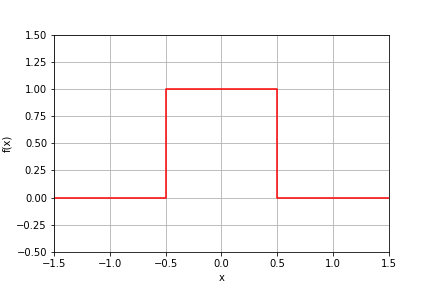
\includegraphics[width=.32\linewidth]{graphics/convolution/convolution_continuos_f_gebs.png}
    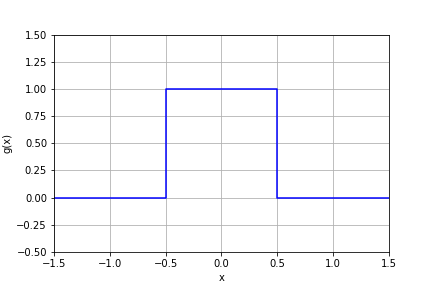
\includegraphics[width=.32\linewidth]{graphics/convolution/convolution_continuos_g_gebs.png}
    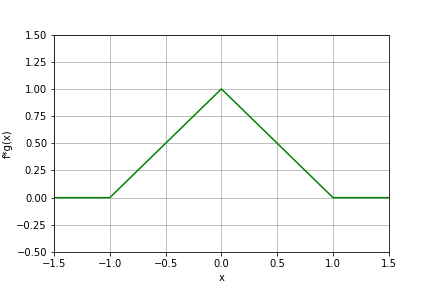
\includegraphics[width=.32\linewidth]{graphics/convolution/convolution_continuos_fg_gebs.png}
    \caption{These plots show two continuous functions ($f(x)$ and $g(x)$) and their convolution $f*g(x)$}
    \label{fig:continuousconvolution}
\end{figure*}
\FloatBarrier
and, for discrete functions $f(n)$ and $g(n)$, as
\begin{equation}
(f * g)(n)\equiv\sum_{m=-\infty}^{\infty}f(m) g(n-m)
\end{equation}
\begin{figure*}[ht]
    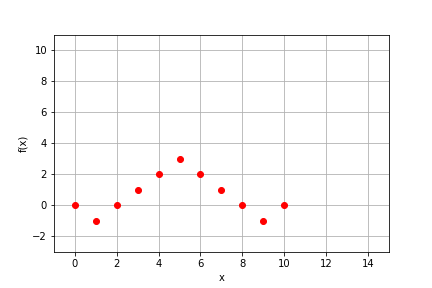
\includegraphics[width=.32\linewidth]{graphics/convolution/convolution_discrete_f_gebs.png}
    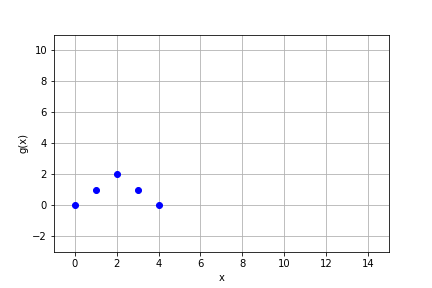
\includegraphics[width=.32\linewidth]{graphics/convolution/convolution_discrete_g_gebs.png}
    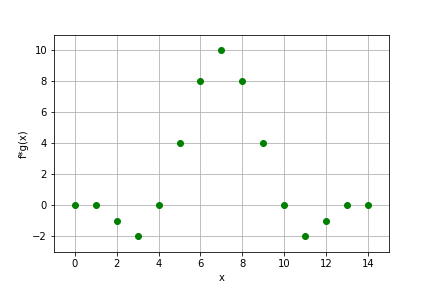
\includegraphics[width=.32\linewidth]{graphics/convolution/convolution_discrete_fg_gebs.png}
    \caption{These plots show two discrete functions ($f(n)$ and $g(n)$) and their convolution $f*g(n)$}
    \label{fig:discreteconvolution}
\end{figure*}
\FloatBarrier
\subsection{Properties}
\label{sec:convolution:mathematics:properties}
\index{convolution!properties}
Since convolution is defined as a product of integrable functions on the linear space, the following algebraic properties are satisfied~\citep{Bracewell2000}:\\
\textbf{Commutativity}
\begin{equation}
(f * g)=(g * f)
\end{equation}
\textbf{Associativity}
\begin{equation}
(f * (g * h))=((f * g) * h)
\end{equation}
\textbf{Distributivity}
\begin{equation}
(f * (g + h))=(f * g) + (f * h)
\end{equation}
\textbf{Multiplication by a scalar value}
\begin{equation}
a (f * g) = (af) * g
\end{equation}
\textbf{Multiplicative identity}, where $\delta$ denotes the delta distribution 
\begin{equation}
f * \delta = f
\end{equation}
\textbf{Differentiation}
\begin{equation}
\frac{d}{dx}(f * g) = \frac{df}{dx} * g = f * \frac{dg}{dx}
\end{equation}
\textbf{Integration}
\begin{equation}
\int_{R^d} (f * g)(x)dx = \bigg(\int_{R^d} f(x)dx\bigg)\bigg(\int_{R^d} g(x)dx\bigg)
\end{equation}
\subsection{Applications}
\label{sec:convolution:mathematics:applications}
\index{convolution!applications}
Listed below are some of the main applications of the convolution operator in various fields of knowledge~\citep{Srivastava2013}:
\begin{itemize}
	\item \textbf{Image Processing} - Different operations are performed on images, in which the original image (larger matrix) and the filter to be applied (smaller matrix, also known as 2D kernel) are treated as 2-dimensional arrays. The kernel size and the values of its elements determine the effect on the original image
    \item \textbf{Signal Filtering} - Provided the filter function is the same as the impulse response function used in in signal filtering, the two operations are equivalent
    \item As a handy tool for \textbf{Polynomial Multiplication} - If we consider two polynomials being multiplied, we can use a convolution process to obtain the coefficients of the resulting polynomial
    \item \textbf{Audio Processing} - Reverberation is a desired effect in auditoriums, music halls, cinemas, and similar constructions. Convolution is used to digitally simulate reverberation in such structures, providing architects with information about the acoustic quality of a building prior to its construction
    \item \textbf{Artificial Intelligence} - Convolutional Neural Networks use convolution in one or more of its internal layers in order to process input data and enhance specific features.
    \item \textbf{Probability Theory} - The Probability Density Function (PDF) of the sum of two independent random variables can be obtained by the convolution of the PDFs of the two variables
\end{itemize}
\index{convolution|)}
\index{convolutional neural networks|(}
\section{Convolution in Neural Networks}
\label{sec:convolution:convolutionalneuralnetworks}
\index{convolutional neural networks!definition}
\subsection{Definition}
\label{sec:convolution:convolutionalneuralnetworks:definition}
Convolutional Neural Networks (CNNs) are a subclass of multi-layer neural networks in which some of its hidden layers are convolutional layers.\\
Like most neural networks, CNNs can be trained using back propagation algorithms and are mostly used to recognize visual patters with minimal or no preprocessing~\citep{Lawrence1997A}.\\
\index{convolutional neural networks!origins and evolution}
\subsection{Origins and Evolution}
\label{sec:convolution:convolutionalneuralnetworks:originsandevolution}
CNNs were initially developed as an attempt to replicate the processing of sight in living organisms.\\
A seminal paper published in 1968~\citep{Hubel1968} noted that two types of neurons took part in the process of identifying images: simple cells (responsible for the detection of straight edges and their orientation), and complex cells (with larger receptive fields, but not affected by the exact position of the edges in the input image).\\
During the 1980s, CNNs evolved, followed by the introduction of Time Delay Neural Networks (TDNNs) in 1987~\citep{Waibel1989}.\\
In the early 1990s, CNNs were modified and used for medical image processing and for automatic detection of breast cancer in mammograms~\citep{Zang1994}.\\
In 1998 LeCun lead a team that created LeNet-5, a CNN used by banks to identify handwritten digits in checks.\\
With the introduction of Graphic Processing Units (GPUs), training of CNNs was greatly improved, allowing for the implementation of efficient Deep Learning Neural Networks with impressive results in image processing and other applications~\citep{Ciresan2013}.
\index{convolutional neural networks!layers}
\subsection{Layers}
\label{sec:convolution:convolutionalneuralnetworks:layers}
A typical CNN has sets of layers with specific functions, such as:
\begin{itemize}
    \item \textbf{Convolutional layer} - This is the main feature of a CNN.\\
    In this layer, a set of filters (also known as kernels) is convoluted over the entire input data. The result of this operation (the activation map of the filter), extracts or enhances specific features in the input data that are passed to the following layers in the CNN.\\
    Since the result of each convolution operation is affected by only a small part of the input data (due to the reduced size of the filter if compared to the size of the input data), this can be interpreted as each point of the activation map being affect by only a small subset of input points.
    \item \textbf{Pooling layer} - In this layer, simple operations are applied in order to reduce the size of the input data, such as maximum pooling or average pooling.\\
    In 2x2 average pooling, for example, each result point the the average of 4 input points, reducing the size of the input field by a factor of 4.
    \item \textbf{Rectified Linear Unit (ReLU) layer} - This layer applies the $f(x) = max(0,x)$ activation function to its input, removing negative values from the input field.
    \item \textbf{Fully Connected layer} - In this layer, usually applied after several convolutional and pooling layers, neurons are connected to all activations in the previous layer, as in regular neural networks.
    \item \textbf{Loss layer} - This is the last layer in a typical CNN. In this layer, training is based on the divergence between the desired and predicted labels.
\end{itemize}
\index{convolutional neural networks!training}
\subsection{Training}
\label{sec:convolution:convolutionalneuralnetworks:training}
One important feature of CNNs is that, with the exception of the Loss layer, all other layers (Convolutional, Pooling, ReLU, and Fully Connected layers) can be trained using unsupervised training~\citep{Arel2010}.\\
Also, usually each layer or set of layers is trained individually, which also improves the speed and the overall result of the training.\\
With the introduction of Graphic Processing Units (GPUs), speed of training and processing in the Convolutional layer has been greatly improved~\citep{Steinkrau2005}
\index{convolutional neural networks!applications}
\subsection{Applications}
\label{sec:convolution:convolutionalneuralnetworks:applications}
CNNs are currently applied to a wide range of areas, such as~\citep{Schmidhuber2015}:
\begin{itemize}
    \item \textbf{Image recognition and Video analysis} - Image Recognition Systems using CNNs are very efficient, specially if applied to facial recognition. Very good results have been obtained in challenges, and in the ImageNetNet tests performed almost as good as humans. If compared to image recognition, video analysis adds a level of complexity, since, in addition to the analysis of each frame, a time dimension needs to be added to the problem and convolution needs to be performed both on each image as well as on the time domain.
    \item \textbf{Game strategy} - A number of board games have been implements using CNNs, most notably Checkers, in Chess and in Go, the first time Artificial Intelligence beat an expert human player in this game.
    \item \textbf{Drug discovery} - In this area, CNNs are used to predict the behaviour of drug molecules and human proteins.
    \item \textbf{Natural language processing} - For NLP, CNNs are used extensively, including semantic parsing, search query retrieval, sentence modeling, classification, and prediction.
\end{itemize}
\index{convolutional neural networks|)}
\index{convolutional filters|(}
\section{Convolutional Filters}
\label{sec:convolution:convolutionalfilters}
\index{convolutional filters!definition}
\subsection{Definition}
\label{sec:convolution:convolutionalfilters:definition}
Convolutional filters (also known as kernels), when applied to image and video processing, are small square matrices with an odd number of rows and columns and used in the Convolutional layer of CNNs in order to detect or enhance specific features in the input image.\\
The convolution operation performed by CNNs is a special two dimensional case of the discrete convolution operator.
\begin{equation}
R(m,n) = (K * I)(m,n)\equiv\sum_{s=-a}^{a}\sum_{t=-b}^{b}K(s,t)I(m-s,n-t)
\end{equation}
where $R(m,n)$ is the convoluted result at point $m,n$, $K$ is the kernel matrix being applied to the input matrix, $I$ is the input matrix, and $a$ and $b$ depend on the dimensions of the kernel used.
\index{convolutional filters!practical example}
\subsection{Practical example: Edge Detection kernel applied}
\label{sec:convolution:convolutionalfilters:practicalexampleedgedetectionkernelapplied}
The figure below shows a practical example of the application of the Edge Detection kernel:
\begin{figure*}[ht]
    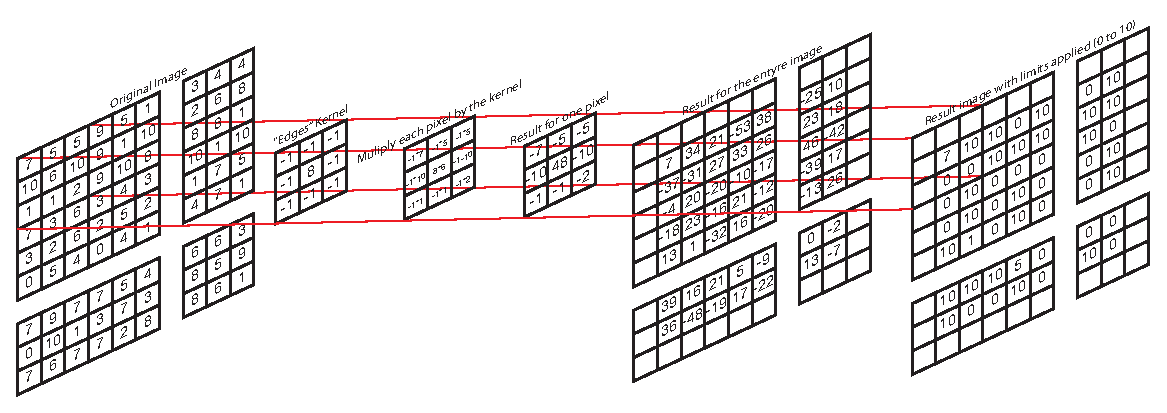
\includegraphics[width=0.90\linewidth]{graphics/convolution/kernel.eps}
    \caption{Edge Detection kernel applied}
    \label{fig:edgedetectionkernelapplication}
\end{figure*}
\FloatBarrier
\begin{itemize}
    \item The kernel is moved over the entire image, pixel by pixel
    \item At each position, the value for each pixel in the original image is multiplied by the corresponding value in the kernel ($7 * -1 = -7$; $5 * -1 = -5$; $5 * -1 = -5$; $10 * -1 = -10$; $6 * 8 = 48$; $10 * -1 = -10$; $1 * -1 = -1$; $1 * -1 = -1$; $2 * -1 = -2$)
    \item All results are added ($(-7) + (-5) + (-5) + (-10) + 48 + (-10) + (-1) + (-1) + (-2) = 7$)
    \item Optionally, the result of the summation may be limited to valid values (colors in images typically range from 0 to 255. In this example we have limited the values to $[0-10]$)
\end{itemize}
\index{convolutional filters!common filters}
\subsection{Common Convolutional Filters}
\label{sec:convolution:convolutionalfilters:commonconvolutionalfilters}
Convolutional filters can be defined to achieve a large range of effects in the input image.\\
A small sample of possible kernels is provided below:
\index{convolutional filters|)}
\begin{figure}[ht]
\begin{minipage}[b]{0.5\linewidth}
\centering
    $$
    \quad
    \begin{bmatrix} 
    0 & 0 & 0 \\
    0 & 1 & 0 \\
    0 & 0 & 0
    \end{bmatrix}
    $$
\caption{\textbf{Identity} Kernel and the original image (unchanged, no convolution applied)}
\end{minipage}
\begin{minipage}[b]{0.3\linewidth}
\centering
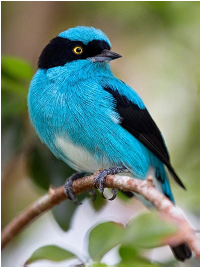
\includegraphics[width=1in]{graphics/convolution/Convolution_gebs_KernelIdentity.png}
\end{minipage}
\label{fig:Identity Kernel}
\end{figure}
\FloatBarrier
\begin{figure}[ht]
\begin{minipage}[b]{0.5\linewidth}
\centering
    $$
    \frac{1}{16}
    \quad
    \begin{bmatrix} 
    1 & 2 & 1 \\
    2 & 4 & 2 \\
    1 & 2 & 1
    \end{bmatrix}
    $$
\caption{\textbf{Gaussian Blur} Kernel and the resulting image}
\end{minipage}
\begin{minipage}[b]{0.3\linewidth}
\centering
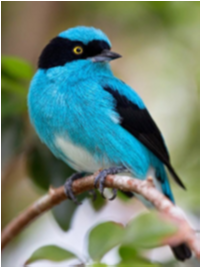
\includegraphics[width=1in]{graphics/convolution/Convolution_gebs_KernelGaussianBlur3x3.png}
\end{minipage}
\label{fig:Gaussian Blur Kernel}
\end{figure}
\FloatBarrier
\begin{figure}[ht]
\begin{minipage}[b]{0.5\linewidth}
\centering
    $$
    \frac{1}{9}
    \quad
    \begin{bmatrix} 
    1 & 1 & 1 \\
    1 & 1 & 1 \\
    1 & 1 & 1
    \end{bmatrix}
    $$
\caption{\textbf{Box Blur} Kernel and the resulting image}
\end{minipage}
\begin{minipage}[b]{0.3\linewidth}
\centering
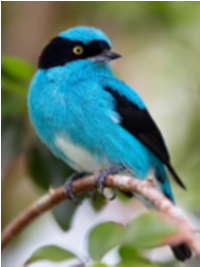
\includegraphics[width=1in]{graphics/convolution/Convolution_gebs_KernelBoxBlur.png}
\end{minipage}
\label{fig:Box Blur Kernel}
\end{figure}
\FloatBarrier
\begin{figure}[ht]
\begin{minipage}[b]{0.5\linewidth}
\centering
    $$
    \frac{-1}{256}
    \quad
    \begin{bmatrix} 
    1 & 4 & 6 & 4 & 1 \\
    4 & 16 & 24 & 16 & 4 \\
    6 & 24 & -476 & 24 & 6 \\
    4 & 16 & 24 & 16 & 4 \\
    1 & 4 & 6 & 4 & 1
    \end{bmatrix}
    $$
\caption{\textbf{Unsharp} Kernel and the resulting image}
\end{minipage}
\begin{minipage}[b]{0.3\linewidth}
\centering
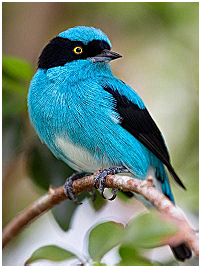
\includegraphics[width=1in]{graphics/convolution/Convolution_gebs_KernelUnsharp5x5.png}
\end{minipage}
\label{fig:Unsharp Kernel}
\end{figure}
\FloatBarrier
\begin{figure}[ht]
\begin{minipage}[b]{0.5\linewidth}
\centering
    $$
    \quad
    \begin{bmatrix} 
    0 & -1 & 0 \\
    -1 & 5 & -1 \\
    0 & -1 & 0
    \end{bmatrix}
    $$
\caption{\textbf{Sharpen} Kernel and the resulting image}
\end{minipage}
\begin{minipage}[b]{0.3\linewidth}
\centering
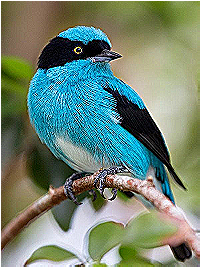
\includegraphics[width=1in]{graphics/convolution/Convolution_gebs_KernelSharpen.png}
\end{minipage}
\label{fig:Sharpen Kernel}
\end{figure}
\FloatBarrier
\begin{figure}[ht]
\begin{minipage}[b]{0.5\linewidth}
\centering
    $$
    \quad
    \begin{bmatrix} 
    -1 & -1 & -1 \\
    -1 & 8 & -1 \\
    -1 & -1 & -1
    \end{bmatrix}
    $$
\caption{\textbf{Edge Detection} Kernel and the resulting image}
\end{minipage}
\begin{minipage}[b]{0.3\linewidth}
\centering
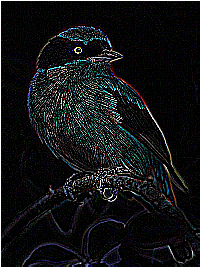
\includegraphics[width=1in]{graphics/convolution/Convolution_gebs_KernelEdgeDetection.png}
\end{minipage}
\label{fig:Edge Detection Kernel}
\end{figure}
\FloatBarrier

\input{terms/crossvalidation_lmd.tex}
\input{terms/dimensionalityreduction_sc.tex} 
\input{terms/ensemblemethods_dv.tex}
\input{terms/lstm_nm.tex}
    \chapter[Neural Networks]{Neural Networks}
\label{ch:neural-networks}\index{Neural Networks|(}
Neural Networks (NNs) are the product of various academic facets, the most prominent one being neuroscience as the structure of a neural network mimics the computation done by the human brain, which makes use of neurons to perform complex calculations such as object recognition from visual input of the eyes. This process is very inefficient to be performed on a computer due to its computational difficulty, which is remedied by the neural network's parallel nature. Neural Network learns with a supervised approach, supplying the model with training datasets in order to adjust the synapses to match the output. The trained model can then be used on unseen data to produce predictions \citep{GURESEN2011426}.

The way the brain trains its neurons is through experience and thus creating a learning process, and neural networks are designed to work the same way by creating synthetic nodes which will behave like organic neurons. Since this structure makes use of learnt experiences, the progress is stored in the form of weighted values at the synapse of each node \citep{Haykin:1994:NNC:541500}.

\section{Types of Neural Networks}

\subsection{Artificial Neural Network}\label{sec:Artificial Neural Network}
An Artificial Neural Network\index{Artificial Neural Network} (ANN) (see Figure~\ref{fig:annfig}) can be defined as a collection of Machine Learning\index{Machine Learning} techniques that together are able to process complex inputs into meaningful spaces or classifications without any further input from the user (such as rules). The ANN is a network of layers, where every node is connected to each node of the previous and next layers. A common setup for an ANN will have an input layer, hidden layer and output layer. Neural Networks are capable of solving both regression (continuous label) and classification (discrete classes) problems, although the main purpose of using these models are for classification purposes, which is highly influenced by the number of nodes in the output layer \citep{Devulapalli2015}.

With regards to hyperparameters, the neural network contains parameters that require many trial and error to discover their optimal value. One of which is the number of hidden layers and nodes, as a small value can result in underfitting and the model would not have enough complexity to learn the dataset, and a large number will result in overfitting, where the model would be able to learn the dataset by rote. The latter is a very common issue with neural networks and can be mitigated with dropout procedure. This method assigns a probability to each node during training in order to periodically deactivate it, thus eliminating the possibility of the next node to base its calculations on the deactivated node, thus eliminating overfitting \citep{Srivastava:2014:DSW:2627435.2670313}.

Another hyperparameter is the learning rate, which is used as a scale to which the model updates its weights. The learning rate should not be very large, as this could overshoot the local minimum and never converge. The ideal way is to use a decaying learning rate in order to alleviate the problems of having a large learning rate as well as small, while still keeping their benefits \cite{jacobs1988increased}. One method to find out hyperparameters is to perform Bayesian Optimization, which builds a probability model on the dataset and selects the hyperparameters with the best score \cite{eggensperger2013towards}. 

As the ANN is traversed, an activation function is fired at each step. Activation functions\index{Activation functions} form the output behaviour of each of the neurons, by applying a specific function to the input nodes and producing the desired output. The activation function may contain a numerical bias\index{bias}, which will transform its output upwards or downwards \citep{jain1996artificial}. Examples of activation functions are as follows:
\begin{itemize}
	
	\item\textbf{Sigmoid function}:
	\begin{marginfigure}%
		\includegraphics[width=\linewidth]{neural_network/sigmoid}
		\caption{The sigmoid function.}
		\label{fig:sigfig}
	\end{marginfigure} The Sigmoid function\index{sigmoid function} is an improvement over the step function as it smoothens out the steep change between the two states. This function maps the input to a value between 0 and 1, both ends being an asymptote\index{asymptote}. The Sigmoid function shown in Figure~\ref{fig:sigfig} is as follows \citep{Haykin:1994:NNC:541500}: $$f(x) = \frac{1}{1+e^{-x}}$$
	
	\item\textbf{Hyperbolic Tangent function}:
	\begin{marginfigure}%
		\includegraphics[width=\linewidth]{neural_network/Tanh}
		\caption{The Tanh function.}
		\label{fig:tanhfig}
	\end{marginfigure}
	The Hyperbolic Tangent function\index{Hyperbolic Tangent function}\index{Tanh} (Tanh) is very similar to the Sigmoid function, with a more stable gradient and an asymptotic range between -1 and 1, thus including negative values. The function shown in Figure~\ref{fig:tanhfig} is the following \citep{Abdelsalam:2017:AEH:3020078.3021768}: $$tanh(x) = \frac{2}{1+e^{-2x}}-1 $$
	
\end{itemize}
The traversal goes from input nodes to the output nodes, and the output will be a mapped function of the input, firing activation functions\index{activation function} at each step. Before performing any predictions, the ANN needs to be trained with labelled data in order to adjust the synapses to their optimal values to form the mapping \citep{GURESEN2011426}. 

The goal of the learning process is to minimize the output of a cost function\index{cost function}, taking into consideration the error value. Each time the input is fed forward through the network, the error of the predicted output is compared to the actual output and thus produce an error value. The cost function $C(n)$, in terms of error $e_k(n)$ is defined as $C(n) = \frac{1}{2}e^2_k(n)$.The error delta in terms of weight $w_{kj}$ is calculated with the following formula: $\Delta w_{kj}(n) = \alpha e_k(n)x_j(n)$ where $\alpha$ is the learning rate\index{learning rate}, $e_k(n)$ is the error and $x_j(n)$ is the input.  \citep{doi:10.1080/02626669809492102}. 

Back-propagation\index{backpropagation} is the process where the biases are updated by distributing the error from the layer closest to the output inwards, applying the derivative of the activation function in the process. The synapses are updated by adding the calculated delta to the weight, formally, $w_{kj}(n+1) = w_{kj}(n) + \Delta w_{kj}(n)$ where $w_{kj}(n)$ is the previous weight and $\Delta w_{kj}(n)$ is the calculated weight difference \citep{Rosen:1994:THL:326619.326741}. Each layer will calculate the error based on the previous error calculations and this will cause a diminishing effect on the error value, leading towards the vanishing gradient problem. \citet{Hochreiter:1998:VGP:353515.355233} points out that this will cause the calculated error delta to be so small that the improvement will be nearly negligible, thus causing the model to be under-trained. One of the remedies to the above phenomenon is to implement Long short-term memory to the model. As the ANN performs epochs, the error of the synapses will converge towards the optimal value, which once reached, the model will be trained. Once the model is trained, one can perform predictions by passing an input through the network and observing the output \citep{Tasdemir:2008:PSR:1500879.1500925}.
\begin{figure}
	\begin{center}
		
	
	\includegraphics[width=0.7\linewidth]{neural_network/ANN}
	%  \checkparity This is an \pageparity\ page.%
	\caption[ANN][6pt]{This diagram is a visual representation of an ANN.}
	\label{fig:annfig}
	%\zsavepos{pos:annfig}
\end{center}
\end{figure}

\subsection{Convolutional Neural Network}\label{sec:Convolutional Neural Network}\index{Convolutional Neural Network}
A Convolutional Neural Network (CNN)(see Figure~\ref{fig:cnnfig})\index{Convolutional Neural Network} is a variant of ANN and are commonly used for image processing and recognition. A CNN usually is a multi-layered network, where each layer will apply a specific function to an image \citep{NIPS2012_4824}. A CNN can use different kinds of layers, each with their own function and output, for example:
\begin{itemize}
	\item\textbf{Features\index{Feature}}: The images are reduced to similar patterns, where each pattern is a small subset of the image and is present in both images \citep{rohrer_2016}.
	\item\textbf{Convolutions}: A filter is applied across every pixel to calculate the similarity between the filter (also referred to as a kernel) and the sample with a convolution function\index{Convolution}. This will output a value that represents the likeness of the feature to the image; the higher the number, the higher the similarity \citep{Alwani:2016:FCA:3195638.3195664}.
	\item\textbf{Average/Max Pooling}: This process\index{Pooling} shrinks the images while still keeping its important features. A small window which is typically 2x2 iterates over pixels, stepping a specific number of pixels each time to possibly avoid overlapping calculations. The output of this filter is the maximum or average value inside the window \. Pooling greatly helps to reduce the computational overhead of processing a large number of pixels and thus converge in less time \citep{Fei:2018:RSP:3240876.3240919,Ciresan:2011:FHP:2283516.2283603}.
	\item\textbf{Rectified Linear Units}: A Rectified Linear Unit\index{Rectified Linear Unit} (ReLU) is considered as an activation function, in that the output is filtered to contain only positive values. This function sets all negative values to 0 and ignores positive ones. This is used to prevent learned values from lingering close to 0 or becoming such a large negative number that it will inhibit the performance \citep{Han:2017:DCN:3055635.3056609}.
	\item\textbf{Fully-Connected Layer}: A fully-connected layer\index{Fully-Connected Layer} (FC) treats the input as a singular list of nodes where each node is connected to all the previous nodes. Each node contains a weighted value which determines the contribution to a specific category when the node is fired. When the layer is activated, the nodes go through a voting process, where each node will vote to which category the input image falls under. The weights will determine which nodes will have more impact in the voting process, and the category with the bigger value of votes will classify the image \citep{Xie:2017:ESA:3160927.3122788}.
	
	\begin{figure}[h]
		\includegraphics[width=\linewidth]{neural_network/CNN}%
		\caption{A diagram of a CNN with deep learning.}%
		\label{fig:cnnfig}%
	\end{figure}
\end{itemize}

A CNN can have multiple repetitions of a set of layers, which will form a deep learning\index{deep-learning} model with a multitude of layers that will eventually produce a final classification of the image. Training of a CNN occurs by feeding the network labelled data and adjusting the weights and features during a backpropagation\index{backpropagation} step, distributing the error and converging to a set error threshold, similar to how ANNs perform their training \citep{Iizuka:2016:LCJ:2897824.2925974}.
\index{Neural Networks|)}
\input{terms/noiseindatasets_is.tex}
\input{terms/onlinelearning_df.tex}
\input{terms/regularisationofmodels_ja.tex}
\chapter[Sample Selection Bias]{Sample Selection Bias}
\label{ch:sample-selection-bias}\index{sample selection bias|(}

    In traditional statistics, the algorithms assume that the the data samples are being drawn in line with the same distribution, and different classes and values of data should appear with roughly the same frequency that they actually occur in the real world. However, this is rarely the case and results in the data becoming biased, meaning that the method of sample collection favours a particular type of data, skewing the distribution of the values \citep{CuddebackEtAl2004}.

    There could be a number of reasons as to why this bias occurs \citep{Tommasi2017}, such as:

    \begin{enumerate}
        \item It might be costly or unpractical to collect certain data.
        \begin{itemize}
        	\item For example, measuring spending habits of large groups of people would be cumbersome, and these people may not necessarily give accurate information.
        \end{itemize}
        \item The entity collecting the data only has access to data belonging to a particular class.
        \begin{itemize}
        	\item For example, if a doctor only has access to patients that are sick, a large portion of the sample would represent sick patients, whereas in relation to the total population the number of sick people would be relatively much smaller.
		\end{itemize}        
        \item Confirmation bias\index{sample selection bias!confirmation bias}, whereby people tend to recall only examples that confirm their existing beliefs.
        \item Incorrect sampling techniques \citep{Marshall1996}, such as sampling from the top of a list instead of randomly
        \item Sampling using results generated from another process.
        \begin{itemize}
        	\item For example, if a system is being trained on detecting fraudulent transactions, and some of these transactions were classified incorrectly by another process, then the model will be trained on false data.   
   		\end{itemize}
    \end{enumerate} 
    
    
    An interesting example that tends to happen within Maltese populations is that related with politics. When a political party passes an online poll regarding a particular issue, the results always tend to be in its favour. This stems from the fact that even though the poll is open to the general public, the outreach of the poll would be much more inclined to reach people within the party - they would have subscribed to social media and news pages, and would regularly follow or check up on their articles and news.
    
    \section{False Information created by Selection Bias}
    
	Having selection bias within a dataset can create false information which does not exist in the actual population, and can lead to inaccurate estimates of the relationships between variables \citep{CuddebackEtAl2004}.
	
	For example, assume a college accepts students that either have high math skills or high science skills. Therefore if a student in this college does not have high math skills, then he must instead have high science skills. This means that a negative correlation between maths and science skills has been created, which does not represent the actual population.
	
	
	\section{How To Prevent Selection Bias}
	
	When collecting a sample of data, one should be attentive in order to prevent selection bias occurring in the dataset. This step of preventing bias is important as not only could it skew the results, but might end up rendering the analysis and conclusions gained from the dataset as useless.
	
	\subsection{Stratified Sampling}\index{sample selection bias!stratification}
	
	This process involves splitting the population into sub-populations before selecting, in order to ensure that an adequate number from each group is selected. For example, splitting a population into age categories and selecting a number from each category \citep{KrautenbacherEtAl2017}
	
	\begin{figure}[hbt!]
	\centering
  		\includegraphics[width=0.88\linewidth]{graphics/sample_selection_bias/Stratified_Diagram.png}
  		\caption{Stratified sampling: splitting the population into categories and selecting accordingly}
  		\label{fig:stratified-sampling}
	\end{figure}
	
	
	\subsection{Not Self Selecting}
	
	Draw from a sample that is not self selecting. If the sample is self-selected, people who are willing to volunteer may share similar characteristics (such as be more outgoing and extroverted), which will create a bias.
	
	\subsection{Analyze Dropouts}	
	
	Determine factors affecting drop outs and establish that no differences exist between participants and non-participants. If those refusing to participate all belong to a certain category, this will create a bias and results need to be corrected to account for these differences \citep{AlonsoEtAl2006}.
	
	\subsection{Sufficient Sample Size}
	
	Ensure a large enough sample size. If the sample size is too small, it will make it more difficult to create an accurate representation.
	
	
	\section{Detecting Selection Bias within a Dataset}
	
	Once data has been collected, or when working on a dataset gained from a different source, it is important to determine whether any sample selection bias exists within the dataset before performing analysis or drawing any conclusions. The processes mentioned below are some methods which can be useful in the detecting such bias.
	
	\subsection{Comparing Distributions}\index{sample selection bias!distribution}
	
	If it is possible to capture information regarding distribution about the whole population, one may then compare this with the sample population. If the distribution if drastically different, it will indicate that a sample selection bias is present.
	
	\begin{marginfigure}
	\centering
  		\includegraphics[width=\linewidth]{graphics/sample_selection_bias/Distributions.png}
  		\caption{Comparing Distributions}
  		\label{fig:comparing-distributions}
	\end{marginfigure}

As a simple example, if the total population contains 50\% males and females, whilst your sample contains 75\% males and 25\% females, it will indicate a selection bias which will skew the results.

Techniques exist to allow the comparison of distributions and measuring the the difference, such as Bayesian Analysis, Kolmogorov--Smirnov test or Chi-Squared test. \citep{GriffinEtAl2013}

	\subsection{Two Step Estimator}\index{sample selection bias!two-step estimator}
	
	This method, as defined by \citet{Heckman1979}, comprises the use of two multiple regression models:
	
	\begin{itemize}
		\item One model is used to examine the interest of the study.
		\item The other regression model is used to detect selection bias and to statistically correct the substantive model. The independent variable could be set to represent participation. The  dependent variable could represent different related statistics.
	\end{itemize}
	
	\subsection{Two Step Estimator Example}
	
	Imagine a survey aiming to collect information about European citizens quality of life. This would include factors such as job status, salary, level of eduction, country GDP, amongst others.
	
The first model would simply use these factors to create a model determining each citizens overall quality of life.

The second model would then measure relationships between participation and other variables. If for example a positive correlation exists between level of education and participation, then a bias in the study has occurred whereby those with a lower level of eduction are being underrepresented.

	\begin{figure}[hbt!]
	\centering
  		\includegraphics[width=0.88\linewidth]{graphics/sample_selection_bias/Education_Correlation_Graph.png}
  		\caption{Two Step Estimator: Using regression models to determine correlations between participants and non-participants}
  		\label{fig:correlation}
	\end{figure}
	
	\section{How to Deal With Selection Bias}
	
	If presented with a dataset which contains selection bias but which cannot be changed or modified due to a number of reasons, then adequate measures should be taken to either mitigate the bias or account for it in the results.
	
	
	\subsection{Post-stratification}\index{sample selection bias!stratification}
	
	In an attempt to make the results more representative of the total population, higher weightings are given to the lower class. If say a sample contains 25\% women, but the general population has 50\%, then you could adjust the estimates by assigning women in the sample higher weights \citep{HoltSmith1979}.
	
As explained by \citet{CortesEtAl2008}, the generalization error \textit{R} on the newly weighted sample is defined as follows:
	
	\begin{equation}\label{weighted_error_function}
    R(h) = \sum_{i=1}^m w_ic(h,z_i)
	\end{equation}
	
	Where \textit{m} is the number of samples, \textit{h} is the error value, \textit{w} is the weight, \textit{c} is the cost function and \textit{z} is the sample value.
	
	\subsection{Synthetic Minority Oversampling TEchnique (SMOTE)}\index{sample selection bias!smote}
	
	Another method of dealing with imbalanced classes is that of generating synthetic data that closely resembles the underrepresented class. In cases where the majority class greatly outweigh the minority class, having a larger dataset that more closely resembles the minority class will balance the results generated.
	
	The way this process works is that new samples are created by finding the midpoint between the line segments joining the existing samples within the minority class.	
	
	\begin{figure}
	\centering
  		\includegraphics[width=0.88\linewidth]{graphics/sample_selection_bias/Smote.png}
  		\caption{SMOTE: generating synthetic samples of the minority class}
  		\label{fig:correlation}
	\end{figure}
	
	SMOTE may also create certain drawbacks. Since the synthetic results are generated on a small set of existing features, it may create an overfitting scenario which might not be able to correctly classify the true outlier nature of the minority class.
	SMOTE might also skew the distribution of the dataset which could affect certain analysis. The large addition of additional samples could also slow down learning speed.\citep{Weiss2007}
	
Studies seem to have shown that using SMOTE techniques to over-represent the minorty class, as opposed to under-representing the majority class by selecting fewer, tends to perform better \citep{ChawlaEtAl2002}. 


	\subsection{Applicability Disclosure}
	
	Giving full disclosure: If it is not possible to eliminate the selection bias from the dataset, then it is important to fully disclose who exactly the results and knowledge gained from the data are applicable to.

\index{sample selection bias|)}

\newcommand{\R}{\mathbb{R}}

\chapter[Semi-Supervised Learning]{Semi-Supervised Learning}
\label{ch:semisuper}

\index{Semi-Supervised Learning|(}

\newthought{Supervised learning} involves a labelled data\index{labelled data}set\index{labelled dataset} on which a classifier\index{classifier} is trained. Once trained, it is then used to predict the labels of similar unlabelled data. Unsupervised Learning\index{Unsupervised Learning} deals with the identification of patterns in a given unlabelled dataset\index{unlabelled dataset}.

Semi-supervised learning lies somewhere in between these two techniques, blending them together. It makes use of both labelled and unlabelled data and is often used in applications where labelled data is difficult to come by. The goal of the semi-supervised classification method is to train a classifier\index{classifier} on both labelled and unlabelled data, with the aim of getting a better result than that provided by a supervised classifier\index{classifier} \citep{zhu2009introduction}.\sidenote{It is also worth noting that semi-supervised methods do not exist only for classification, but also for regression\index{regression} problems.}

\section{Semi-Supervised Classification and Clustering}\label{sec:class_clust}

\newthought{Similar to Supervised Learning\index{Supervised Learning}}, Semi-Supervised Learning can be split into two categories; Semi-Supervised Classification\index{Semi-Supervised Classification} and Semi-Supervised Clustering\index{Semi-Supervised Clustering}. We now take a closer look at each of these two areas.

\subsection{Semi-Supervised Classification}\label{sec:class}

\newthought{Semi-Supervised Classification} is a classification\index{classification} problem which makes use of both labelled and unlabelled data in the same dataset. As is typical of such a problem, we assume that the volume of unlabelled data in the dataset is larger than that of labelled data.

In semi-supervised learning, we make use of Pseudo-Labelling\index{Pseudo-Labelling} \citep{lee2013pseudo} to increase the amount of labelled data\index{labelled data} upon which the classifier\index{classifier} is being trained. The process is as follows:

\begin{enumerate}
\item We first use the smaller portion of labelled data\index{labelled data} to begin training our model.
\item We then use this model to predict the labels for the unlabelled data in the dataset.
\item The model is re-trained on all of the labelled data\index{labelled data}, including the original labelled entries as well as the new pseudo-labelled\index{pseudo-label} entries.
\item Steps 2 and 3 are then repeated for any unlabelled data left (if any).
\end{enumerate}

Hence in this way, semi-supervised classification offers the same performance as a Supervised Classification\index{Supervised Classification}, with the added benefit that the unlabelled data is automatically labelled by the classifier\index{classifier} itself, reducing the effort needed for manual labelling in the dataset. 

\subsection{Semi-Supervised Clustering}\label{sec:clust}

\newthought{Semi-Supervised Clustering}, also known as Constrained Clustering\index{Constrained Clustering}, can be considered as a supervised extension added to Unsupervised Clustering\index{Unsupervised Clustering} \citep{zhu2009introduction, bradley2000constrained}. 

In such a case, the dataset in question consists of unlabelled data, the same as a typical Unsupervised Clustering\index{Unsupervised Clustering} problem. Distinctively however, in Constrained Clustering\index{Constrained Clustering} one also finds a degree of supervised information about the data clusters\index{clusters} inside of the dataset. Such information may contain constraints such as \textit{must-link}\index{must-link} and \textit{cannot-link}\index{cannot-link}, where in the former, two data elements $x_i$ and $x_j$ must be in the same cluster, while in the latter they must not \citep{zhu2009introduction}. Using Constrained Clustering\index{Constrained Clustering} we aim at clustering\index{clustering} better than a typical unsupervised clustering technique.

\section{Method}\label{sec:method}

\newthought{Initially, it may seem illogical} that a semi-supervised process making use of unabelled data can perform as good as or better than a supervised labelled solution. Unlabelled data is incapable of providing a relationship between an element $x$ and a label $y$, which is what a Supervised Model is trained upon. What gives Semi-Supervised Learning its strength is the assumptions made between the unlabelled data and the target labels\index{target label}.

To examine the discussed process, let us take an example proposed by \citet{zhu2009introduction}. First we represent each data instance\index{data instance} by a one-dimensional feature $ x \in\R$. $x$ can be in one of two classes; positive or negative.

\begin{itemize}
\item In a case of Supervised Learning\index{Supervised Learning}, we are given the labelled training instances $(x_1,y_1) = (-1, -)$ and $(x_2, y_2) = (1,+)$. In such a case the best Decision Boundary\index{Decision Boundary} would be $x = 0$, where all instances having $x < 0$ are classified as $y = -$, and those having $x \geq 0$ as $y=+$.
\item Now let us consider also a large number of unlabelled instances with unknown correct class labels\index{class label}. We observe however, that they form two groups. Taking the assumption that instances in each class form a coherent group\index{coherent group}, we know that instances tend to center around a central mean\index{central mean} in a Gaussian Distribution\index{Gaussian Distribution}. 
\item Through this assumption, the unlabelled data is capable of providing us with more information. We now notice that the two labelled instances\index{labelled instance} detailed in the first point are not the best examples for each of the classes in our dataset.
\item Hence we take a semi-supervised estimate, which shows us that the Decision Boundary\index{Decision Boundary} should be between these two latter groups instead, at $x \approx 0.4$.
\end{itemize}

If the assumption holds, then using both the labelled and unlabelled data gives us a more reliable Decision Boundary\index{Decision Boundary} than the one initially proposed. As we can see from this example (displayed also in Figure~\ref{fig:super_vs_semi}), the distribution of the unlabelled data helps us in identifying the regions having the same label, with the smaller amount of labelled instances\index{labelled instance} providing us with the actual labels.

\begin{figure}
\includegraphics[scale=1]{"graphics/semi-supervised learning/supervised_vs_semi"}
\caption[Supervised vs Semi-Supervised Example][70pt]{An example of the decision boundaries determined by a Supervised system and a Semi-Supervised system.  Source: Zhu \& Goldberg (2009)}
\label{fig:super_vs_semi}
\end{figure}

\subsection{Inductive vs. Transductive Semi-Supervised Learning\index{Transductive Semi-Supervised Learning}}\label{sec:inductive_transductive}

\newthought{In Semi-Supervised Learning}, on finds two modes. Since in our dataset we have both labelled and unlabelled data, we have two goals to achieve, namely:

\begin{enumerate}
\item To predict the labels for the upcoming data instances\index{data instance} in the test set\index{test set}. This is known as \textbf{Inductive Semi-Supervised Learning}.
\item To predict the labels of the unlabelled data instances inside of the training set\index{training set}. This is known as \textbf{Transductive Semi-Supervised Learning}.
\end{enumerate}

Formally, in Inductive Semi-Supervised Learning\index{Inductive Semi-Supervised Learning} \citep{zhu2009introduction}, given a training sample; 

\begin{equation}
\{(\bm{x}_i, y_i)\}^{l}_{i=1},\{\bm{x}_j\}^{l+u}_{j=l+1}
\end{equation}

...our model learns a function $f:X \mapsto Y$, such that $f$ is expected to be a good predictor on future data, beyond $\{\bm{x}_j\}^{l+u}_{j=l+1}$.

In Transductive Learning \citep{zhu2009introduction}, given a training sample;

\begin{equation}
\{(\bm{x}_i,y_i)\}^l_{i=1},\{\bm{x}_j\}^{l+u}_{j=l+1}
\end{equation}

...our model learns a function $f: X^{l+u} \mapsto Y^{l+u}$, such that $f$ is expected to be a good predictor on the unlabelled data $\{\bm{x}_j\}^{l+u}_{j=l+1}$.

\subsection{Limitations of Semi-Supervised Learning}\label{sec:limitations}

\newthought{Semi-Supervised Learning} may seem as a revolutionary step on Supervised Learning\index{Supervised Learning}; providing the same, if not better, performance, while using incomplete datasets with unlabelled data.

In reality however it is not that simple. Blindly opting for Semi-Supervised methods for any specific task can often lead to worse results than a Supervised solution \citep{zhu2009introduction}. 

This is due to the assumption we make when handling the unlabelled data in our dataset. Since our Semi-Supervised model relies heavily on this assumption, a wrong one can lead to a significant decrease in performance and accuracy. Careful evaluation of the data is a must before committing to which type of learning algorithms\index{algorithm} to use.

\section{Semi-Supervised Learning in Algorithms \& Applications}\label{sec:applications}

\newthought{Semi-Supervised Learning} can be found in various practical applications, including i) Image Searching\index{Image Searching}, ii) Genomics\index{Genomics}, iii)Natural Language Processing\index{Natural Language Processing} and iv) Speech Analysis\index{Speech Analysis}. It can be integrated inside of well-known algorithms\index{algorithm}, each of which having its own advantages and disadvantages, and must be used dependently on the application in question.

A simple yet effective algorithm making use of Semi-Supervised Learning is known as the Self-Training Model \citep{mcclosky2006effective, zhu2009introduction}. It is a Wrapper Method\index{Wrapper Method}, capable of wrapping itself around other algorithms\index{algorithm} without altering their inner workings. It also comes with a crucial limitation; small errors occurring in the initial training iterations\index{training iteration} can get reinforced throughout the rest of the training.

To combat this limitation, among other improvements, one also finds other, more complex algorithms\index{algorithm}. Transductive SVMs\index{Transductive SVM} \citep{bennett1999semi} are Support Vector Machines\index{Support Vector Machine} embedded with Semi-Supervised Learning.These methods however have difficulty scaling to large amounts of data. Graph-Based Methods\index{graph-based method} \citep{goldberg2006seeing, zhu2009introduction} are some of the most used techniques. Labelled information\index{labelled information} is spread through the graph from labelled\index{labelled node} to unlabelled nodes, connecting similar observations. One also finds Neural Network\index{Neural Network} solutions such as Generative Models\index{Generative Model} and Deep Generative Models\index{Deep Generative Model} \citep{zhu2009introduction, kingma2014semi}, which are capable of allowing a more robust set of features to be used than Linear Embedding\index{Linear Embedding} used by other solutions.

\index{Semi-Supervised Learning|)}
 
\input{terms/syntheticfeatures_fcm.tex}
\input{terms/transferlearning_jjd.tex}
\input{terms/roccurves_pb.tex} %TODO

%%
% The back matter contains appendices, bibliographies, indices, glossaries, etc.

\backmatter

\bibliography{terms/bayesianmodels_kj,terms/neuralnetwork_bp,terms/roccurves_pb,terms/dimensionalityreduction_sc,terms/semisupervised_mm,terms/lstm_nm,terms/regularisationofmodels_ja,terms/transferlearning_jjd,terms/sampleselectionbias_ac,terms/noiseindatasets_is,terms/onlinelearning_df,terms/crossvalidation_lmd,terms/confusionmatrix_df,terms/activationfunctions_km,terms/syntheticfeatures_fcm,terms/ensemblemethods_dv,terms/convolution_gebs} %TODO
\bibliographystyle{plainnat}

\printindex

\end{document}
